\documentclass[12pt, a4paper]{article}
\usepackage[french]{babel}
\usepackage{caption}
\usepackage{graphicx}
\usepackage[T1]{fontenc}
\usepackage{listings}
\usepackage{geometry}
\usepackage{pgfplots}

\usepgfplotslibrary{polar}
\pgfplotsset{compat=1.12} 

\pgfplotsset{width=10cm,compat=1.9}
\usepackage[colorlinks=true,linkcolor=black,anchorcolor=black,citecolor=black,filecolor=black,menucolor=black,runcolor=black,urlcolor=black]{hyperref}
\usepackage{fancyhdr}
\pagestyle{fancy}
\lhead{}
\rhead{}
\chead{}
\rfoot{\thepage}
\lfoot{Martin Baumgaertner}
\cfoot{}

\renewcommand{\headrulewidth}{0.4pt}
\renewcommand{\footrulewidth}{0.4pt}

\begin{document}
\begin{titlepage}
	\newcommand{\HRule}{\rule{\linewidth}{0.5mm}} 
	\center 
	\textsc{\LARGE iut de colmar}\\[6.5cm] 
	\textsc{\Large R403 -- physique des télécoms}\\[0.5cm] 
	\textsc{\large Année 2022-23}\\[0.5cm]
	\HRule\\[0.75cm]
	{\Large\bfseries Etat de l'art et fabrication d'un antenne YAGI}\\[0.4cm]
	\HRule\\[1.5cm]
	\textsc{\large martin baumgaertner}\\[6cm] 

	\vfill\vfill\vfill
	{\large\today} 
	\vfill
\end{titlepage}
\newpage
\tableofcontents
\listoffigures
\newpage
\section{Introduction}
\subsection{Définition}
L'antenne Yagi est un type d'antenne directive utilisée 
pour la réception et la transmission de signaux radio. 
Elle se compose de trois principaux éléments. Un reflecteur,
placé à l'opposé du sens de propagation, au milieu, 
un dipôle, puis un directeur qui lui permet d'orienter
le signal.\\

Voici un schéma réprésentatif d'une antenne Yagi :
\begin{figure}[h]
    \centering
    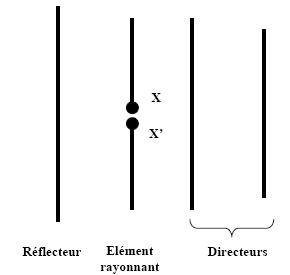
\includegraphics[width=0.5\textwidth]{img/yagi.jpg}
    \caption{Schéma d'une antenne Yagi \cite{r1}}
    \label{fig:yagi}
\end{figure}

\begin{figure}[h]
    \centering
    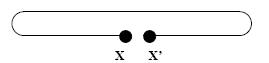
\includegraphics[width=0.5\textwidth]{img/trombone-yagi.jpg}
    \caption{Le dipôle vu de face \cite{r1}}
    \label{fig:yagi-de-face}
\end{figure}

Le dipôle peut être aussi appelé "trombone" en raison de sa
forme. Il est composé de deux éléments de même longueur. 
La longueur du dipôle est lié à la fréquence du signal
que l'on souhaite recevoir/émettre. En effet, la longueur
du dipôle doit être égale au quart de la longueur d'onde 
pour l'antenne Yagi la plus facile à réalisé : la quart d'onde.



\subsection{Présentation}

L'antenne Yagi, également connue sous le nom de 
"râteau", tire son nom de l'ingénieur japonais 
Shintaro Uda de l'université Tohoku à Sendai, qui 
l'a développée en collaboration avec son professeur 
Hidetsugu Yagi. En 1924, Uda conçut cette antenne 
directive, et la première publication sur sa découverte 
eut lieu en 1926 en japonais, puis en 1928 en anglais 
dans la revue scientifique "The Proceedings of the 
Institute of Radio Engineers" aux États-Unis. 
À partir de 1934, les radioamateurs ont commencé à
expérimenter cette antenne.\\

Pendant la Seconde Guerre. mondiale, l'antenne 
Yagi a été largement utilisée pour les radars.
Toutefois, c'est dans les années 50, avec le
développement de la télévision, qu'elle s'est
répandue massivement sur les toits des habitations.
Elle est devenue populaire sous le nom
commun de "râteau", en raison de sa ressemblance.

Ainsi, l'antenne Yagi, de part son origine au Japon et
son utilisation répandue pendant la guerre et l'ère
de la télévision, a joué un rôle significatif dans
l'histoire des communications et continue d'être
utilisée de nos jours.\\

De nos jours les antennes Yagi sont principalement 
utilisées pour la réception de signaux de télévision
terrestre, pour la réception de signaux
radioamateurs et de téléphonie mobile. Ou bien même 
encore pour l'utilisation de Wi-Fi, bien installée, 
l'antenne permet de couvrir un bien plus grande surface 
qu'un petit modem. 


\section{Caractéristiques et propriétés des antennes Yagi}
\subsection{Fréquences et largeur de bande}
La largeur de bande des antennes Yagi est relative 
à l'utilisation que l'on en fait. En effet, la largeur 
de bande pour un réseau Wi-Fi sera bien plus grande
que celle d'une antenne de télévision. Voici quelques 
exemples de largeur de bande pour différentes 
utilisations :\\
\begin{itemize}
    \item Télévision numérique : 470-862 MHz 
    \item Réseaux Wi-Fi : 2,4-5,8 GHz
    \item Radioamateur : varie en fonction des bandes de fréquences souhaitées (HF, VHF, UHF)
\end{itemize}

\newpage
\subsection{Gain et directivité}
Le gain d'une antenne varie en fonction 
du nombre d'éléments qui la compose. En effet, plus
il y a d'éléments, plus le gain est important mais arrivé
à un certain point, le gain ne varie plus. Comme nous 
pouvons le voir ci-dessous, arrivé aux alentours 
de 20 élements on se rend compte que le gain commence
à stagner tout doucement. Il faut savoir adapter le nombre 
d'élements en fonction de ses besoins car cela va venir jouer
sur la directivité du signal. Plus il y a d'éléments directeurs
plus on va venir concentrer l'énégie émise et donc, nous serons
plus précis, et donc la fréquence choisie peut être plus 
précise. À contrario la largeur de bande sera donc réduite.  \\ 

\begin{figure}[h]
    \centering
    \begin{tikzpicture}
        \begin{axis}[	grid= major ,
                width=1\textwidth ,
                xlabel = {Nombre éléments} ,
                ylabel = {Gain(dBi)} ,
                xmin = 1, xmax = 26,
                ymin = 0, ymax = 20,
                legend entries={Évolution du gain},
                legend style={at={(0,1)},anchor=north west}]
            \addplot coordinates {(2, 6) (3, 8) (4, 9) (5, 10) (6, 11) (7, 12) (8, 13) (9, 13) (10, 14) (12, 14) (14, 15) (16, 15) (18, 16) (20, 16) (22, 17) (24, 17)}; % Tracé point à point
        \end{axis}
    \end{tikzpicture}
    \caption{Gain en fonction du nombre d'éléments}
\end{figure}

\newpage
Le nombre d'éléments et le gain est directement correlé 
à la longueur totale du boom. Ce dernier répresente la partie
centrale de l'antenne, c'est sur cette partie que l'on va venir
fixer tous les éléments de l'antenne Yagi perpendiculairement au boom.\\

Sur le tableau qui suit nous pouvons nous rendre compte
de la liaison direct entre le nombre d'éléments et la longueur
du boom.\\

\begin{figure}[h]
    \centering
    \begin{tabular}{|c|c|c|}
        \hline
        Nombre d'éléments & Longueur du boom & Gain \\
        \hline
        3 & 0,4 $\lambda$ & 6 dBi \\
        \hline
        4 & 0,7 $\lambda$ & 8 dBi \\
        \hline
        5 & 1,1 $\lambda$ & 9 dBi \\
        \hline
        6 & 1,4 $\lambda$ & 10 dBi \\
        \hline
        7 & 1,8 $\lambda$ & 11 dBi \\
        \hline
        8 & 2,1 $\lambda$ & 12 dBi \\
        \hline
        9 & 2,5 $\lambda$ & 13 dBi \\
        \hline
        10 & 2,8 $\lambda$ & 13 dBi \\
        \hline
        12 & 3,2 $\lambda$ & 14 dBi \\
        \hline
        14 & 3,9 $\lambda$ & 14 dBi \\
        \hline
        16 & 4,6 $\lambda$ & 15 dBi \\
        \hline
        18 & 5,3 $\lambda$ & 15 dBi \\
        \hline
        20 & 6 $\lambda$ & 16 dBi \\
        \hline
        22 & 6,7 $\lambda$ & 16 dBi \\
        \hline
        24 & 7,4 $\lambda$ & 17 dBi \\
        \hline
    \end{tabular}
    \caption{Corrélation entre le nombre d'éléments, gain et longueur du boom \cite{r2}}
    \label{fig:tableau}
\end{figure}


\newpage
\section{État de l'art des antennes Yagi}
\subsection{Fonctionnement}
L'antenne Yagi est une antenne directive 
utilisée pour la réception de signaux radio et les 
communications sans fil. Elle est constituée d'un 
dipôle, d'un réflecteur et de directeurs. Les ondes 
radio sont propagées par le dipôle. En avant du 
dipôle, les directeurs concentrent l'énergie dans la 
direction désirée, créant ainsi le lobe principal de 
rayonnement. Le réflecteur à l'arrière du dipôle réduit 
la directivité de l'antenne en réfléchissant les ondes 
émises. Pour garantir une performance optimale, les 
dimensions des éléments sont soigneusement calculées en 
fonction de la fréquence voulu. En combinant ces 
composants et leur positionnement de manière approprié, l'antenne 
Yagi peut concentrer l'énergie rayonnée dans une 
direction spécifique, ce qui permet un gain élevé et 
une réception et une transmission améliorées dans 
cette direction.

Voici le diagramme 3D de propagation des ondes 
d'une antenne Yagi, on peut voir que les ondes sont
concentrées dans une direction précise.\\

\begin{figure}[h]
    \centering
    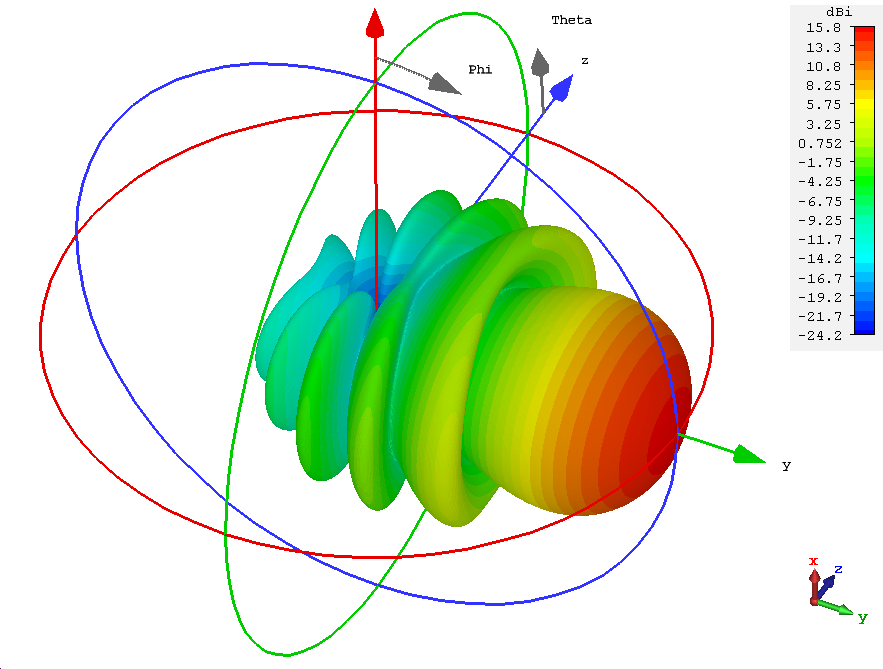
\includegraphics[width=0.9\textwidth]{img/pattern.png}
    \caption{Diagramme 3D de propagation des ondes \cite{r4}}
    \label{fig:3d}
\end{figure}


\subsection{Avantages et limitations}
Les avantages d'une antenne Yagi sont nombreux. Sa directivité
permet de concentrer l'énergie dans une direction précise, 
et donc, une communication sélective. Sa directivité
permet également d'avoir un gain plus élevé que les
antennes omnidirectionnelles. De plus, les antennes 
Yagi sont facilement concevable comme nous le verrons 
dans une partie après, ce qui la rend donc réalisable
par les radioamateurs.\\

Bien que l'antenne Yagi possède de nombreux avantages, ces derniers
peuvent se transformer en inconvénients. En effet, la directivité de l'antenne
lui permet de concentrer l'énergie dans une direction
précise, mais cela implique que l'antenne doit être
orientée dans la direction voulue. De plus, la directivité
de l'antenne implique que la communication ne peut se faire
que dans une direction précise, ce qui peut être un inconvénient
dans certains cas. Dans le cas où nous voudrions fabriquer
une antenne Yagi, il faut être précis et rigoureux dans
les calculs, car la moindre erreur peut avoir un impact. 
Enfin, une antenne Yagi maison sera limité à donc une
largeur de bande, il faudra donc construire plusieurs antennes
si l'on souhaite communiquer sur plusieurs fréquences.\\

\subsection{Une antenne en constante évolution}
L'antenne Yagi est en constante évolution, elle reste 
une des plus utilisées dans le monde est 
est améliorée de jour en jour. En effet, de nombreux 
domaines en ont besoin et est donc améliorée en
fonction des usages requis.\\

De nos jours plusieurs méthodes de simulation
sont utilisées pour améliorer les antennes Yagi à moindre
coût. La méthode des éléments finis est la plus utilisée
car elle permet de simuler le comportement de l'antenne
en fonction d'une mutlitude de paramètres. Cette méthode 
"permet de vérifier l'adéquation de produits 
numériquement avant même leur construction[...]" \cite{r3}.
Elle est particulièrement adaptée pour 
résoudre des problèmes complexes avec des matériaux 
hétérogènes.

Les matérieux utilisés sont eux aussi en constante 
évolution. Désormais, de plus en plus d'aluminium 
est préconisé pour offrir une meilleure résistance 
aux intempéries et un gain de poids non négligeable.

Pour finir, les antennes Yagi sont devenu polyvalentes.
En effet, celles que l'on retrouve dans le commerce
sont désormais multi-bandes. Cela permet de couvrir
plusieurs fréquences avec une seule antenne. L'ajout
de communutateurs d'alimentation permet de choisir
la fréquence que l'on souhaite utiliser.\\





\section{Fabrication d'une antenne YAGI}
Réaliser une antenne Yagi est tout à fait possible, chez 
soit, en utilisant des matérieux de tous les jours. 
Nous allons voir ci-après les étapes à suivre 
pour fabriquer une antenne Yagi maison que l'on 
pourrait utiliser pour la recherche de balise. Sa 
fréquence sera de 121Mhz, et son coût 
une trentaine d'euros. Notre antenne sera constituée
de 3 éléments, un dipôle, un réflecteur et un directeur.
Pour concevoir cette antenne je me suis inspiré et aidé
de l'internaute \textbf{Hugues F4GSN} de la page 
\textbf{Radioamateurs du Haut-Rhin} \cite{r5}.
\subsection{Logiciels de conception et de simulation}
Il existe de nombreux logiciels de conception et de
simulation d'antennes Yagi. Pour essayer notre 
projet et le valider avant de l'essayer nous pouvons 
utiliser \textbf{4NEC2} qui est gratuit et nécessite 
windows. Vu la simplicité de notre antenne, nous
n'avons pas besoin d'utiliser de logiciel de simulation.\\

J'utiliserai cependant un calculateur en ligne \textbf{Yagi Calculator}
qui permet de me donner la longueur du boom, du directeurs 
et de tous les autres éléments de mon antenne. Grâce 
à ce calculateur, je pourrai vérifier mes calculs comme 
nous le verrons ci-après.

\subsection{Formules et équations utiles pour le dimensionnement}
Pour concevoir notre antenne il faut calculer 
les dimensions des éléments. Nous allons 
commencer par calculer la longueur d'onde de notre
antenne. Pour cela nous utilisons la formule suivante :\\

\begin{equation}
    \lambda = \frac{c}{f}
    = \frac{3*10^8}{121*10^6}
    = 2.47m
\end{equation}

\newpage
Une fois notre longueur d'onde trouvé, nous 
pouvons en déduire la longueur approximative du boom 
de notre antenne. Pour ce faire, nous prenons 
mon tableau d'avant, et nous voyons que pour 3 élements
nous divisons d'à peu près 25\% la longueur d'onde. Nous obtenons
donc une longueur de boom de 801mm.\\
Ce calcul est vérifié par le calculateur en ligne 
\textbf{Yagi Calculator} :
\begin{figure}[h]
    \centering
    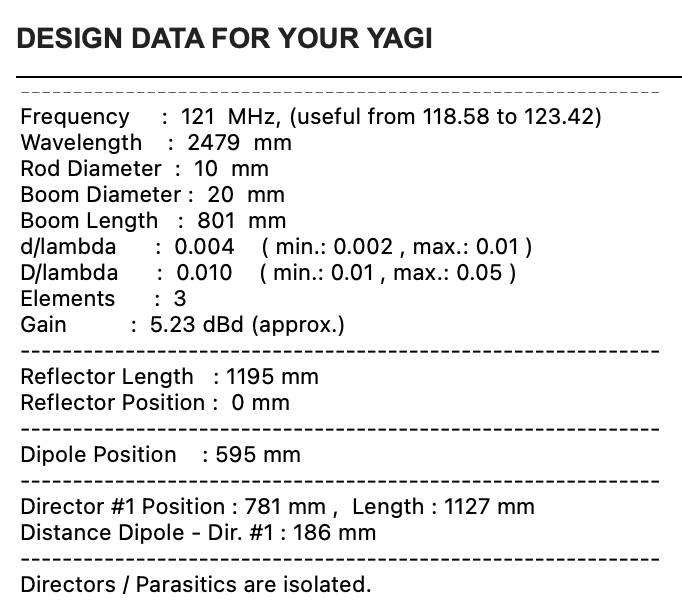
\includegraphics[width=0.5\textwidth]{img/calc.png}
    \caption{Calcul des dimensions de l'antenne}
    \label{fig:calcul}
\end{figure}

Nous retrouvons à peu près les mêmes valeurs sur le schéma
de l'internaute Hugues :
\begin{figure}[h]
    \centering
    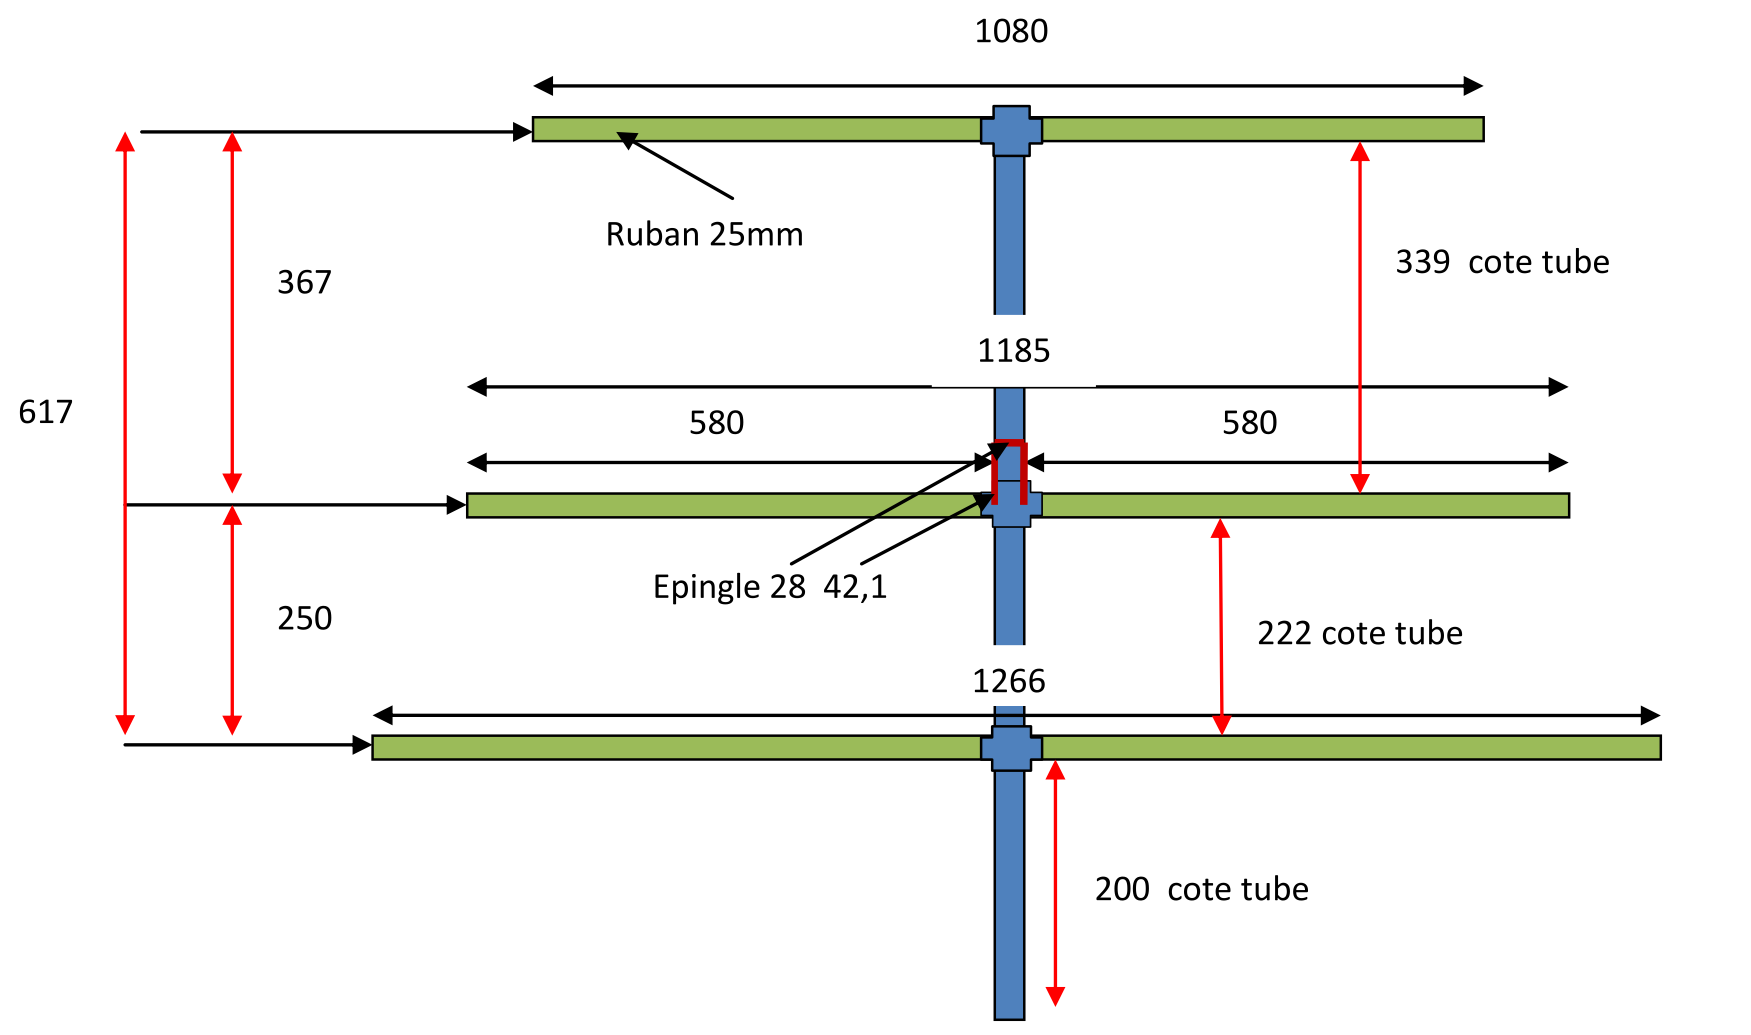
\includegraphics[width=0.7\textwidth]{img/boom.png}
    \caption{Schéma de l'antenne Yagi selon \textbf{Hugues F4GSN}}
    \label{fig:antenne}
\end{figure}

\subsection{Outils et matériaux nécessaires}
Pour réaliser cette antenne il faut se munir 
du matériel suivant :\\
\begin{itemize}
    \item 1m de tube PVC pression DN20 diamètre extérieur 25mm
    \item 1 Té PVC pression DN20 diamètre intérieur 25mm
    \item 2 croix PVC pression DN20 diamètre intérieur 25mm
    \item 0,13m de fil de cuivre nu 1,5 mm² pour faire l’épingle
    \item 3,55m de ruban métallique largeur 25mm (type mètre ruban)
    \item 2m de câble coaxial RG-58 avec fiche selon besoin PL/N/SMA/BNC…
    \item Visserie inox, écrous,rondelles grower (pour les vis 3×15mm ou 3×20mm)
    \item 4 cosses à souder pour la connexion du câble coaxial et de l’épingle
\end{itemize}


\subsection{Fabrication de l'antenne}
\subsubsection{Le boom}
Pour construire l'antenne il faut venir respecter les 
longueur de coupes indiqués sur le schéma fourni 
au milimètre près. Voici les dimensions à respecter 
du tube PVC pour constituer le boom :\\
\begin{itemize}
    \item 1 tube DN20 de 339mm
    \item 1 tube DN20 de 222mm
    \item 1 tube DN20 de 200mm
\end{itemize}
\subsubsection{Les éléments}
Pour les éléments, il faut venir découper le ruban
métallique en fonction des dimensions suivantes :\\
\begin{itemize}
    \item 1 réflecteur de 1266mm
    \item 1 dipôle de 1185mm
    \item 1 directeur de 1080mm
\end{itemize}

\subsubsection{L'épingle}
Pour réaliser l'épingle, il faut installer l'élément le plus
important de l'antenne. Il faut se munir d'un câble 
coaxial de 2m et venir le dénuder sur 10cm. Nous allons 
venir le fixer sur le dipôle à l'aide d'une épingle
en cuivre. Pour cela, il faut venir couper un fil de
cuivre en respectant les valeurs énnoncées un peu plus 
tôt. Ensuite, nous viendrons souder les cosses sur le câble
coaxial et sur l'épingle. Pour finir,
fixerons l'épingle sur le dipôle à l'aide de vis et de
rondelles. Voici le résultat final :\\
\begin{figure}[h]
    \centering
    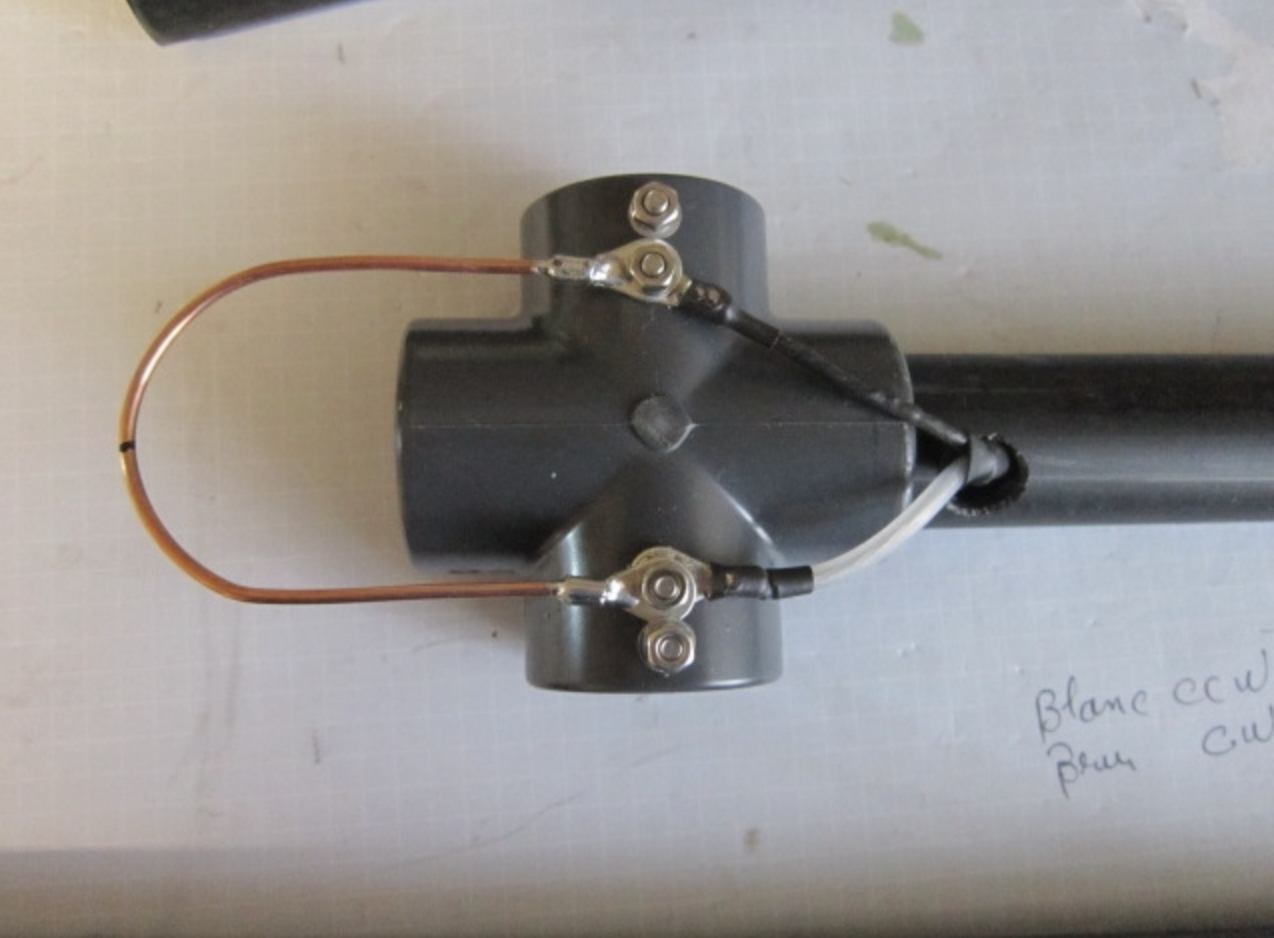
\includegraphics[width=0.7\textwidth]{img/dipole.png}
    \caption{Epingle sur le dipôle \cite{r5}}
    \label{fig:epingle}
\end{figure}

\subsubsection{Le montage}
Pour finir, il suffit d'assembler tous les éléments
en veillant à le câble sur un analyseur d'antenne.
Voici le résultat final par l'internaute Hugues :\\
\begin{figure}[h]
    \centering
    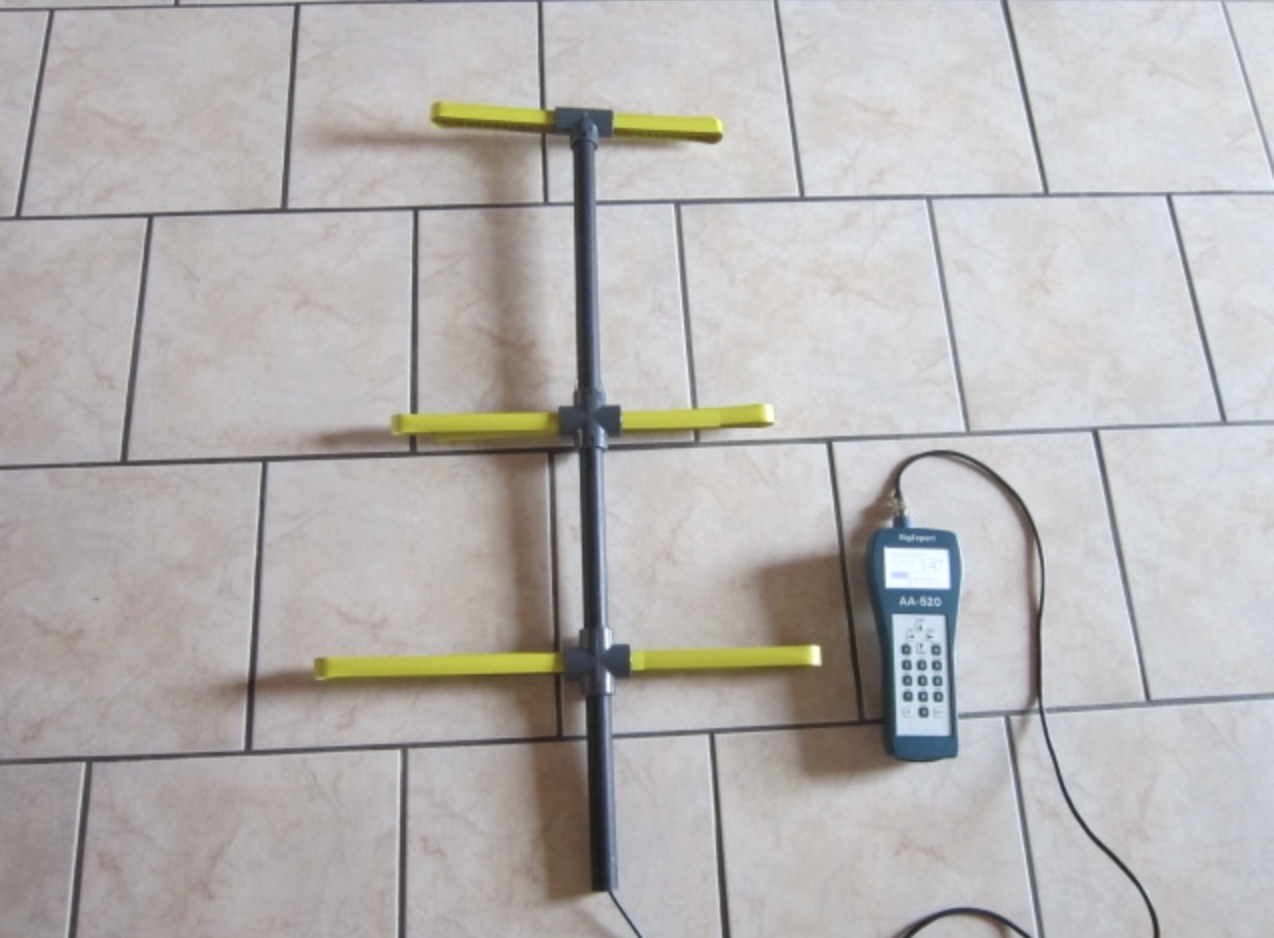
\includegraphics[width=0.5\textwidth]{img/fin.png}
    \caption{Antenne Yagi 3 éléments \cite{r5}}
    \label{fig:fin}
\end{figure}

\newpage
\subsection{Exemples de projets de fabrication d'antennes Yagi}
Comme énnoncé tout au long de ce devoir, il existe
de nombreuses utilisations possibles pour les antennes 
Yagi. Voici quelques exemples de réalisations que 
j'ai pu trouvé. 
\subsubsection*{Antenne Yagi 4 éléments 100Mhz}
\begin{figure}[h]
    \centering
    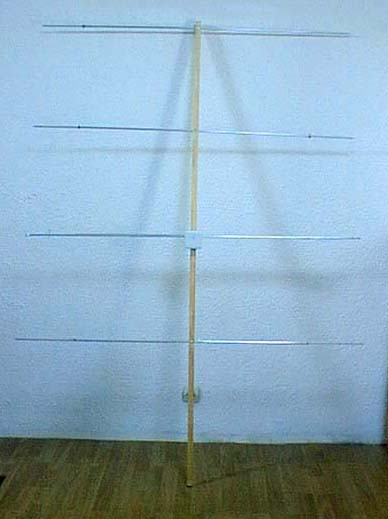
\includegraphics[width=0.5\textwidth]{img/antenne-4.jpg}
    \caption{Antenne Yagi 4 éléments \cite{r6}}
    \label{fig:antenn}
\end{figure}

\subsubsection*{Antenne 2,4GHz pouvant être utilisé pour amplifié le signal Wi-Fi}
\begin{figure}[h]
    \centering
    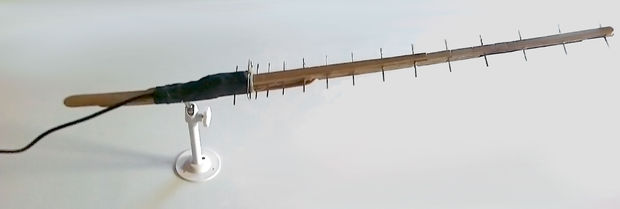
\includegraphics[width=0.5\textwidth]{img/ant-wifi.jpg}
    \caption{Antenne Yagi Wi-Fi \cite{r7}}
    \label{fig:wifi}
\end{figure}




\section{Conclusion}
En definitive, nous avons pu voir au travers 
de ce devoir que les antennes Yagi sont des
antennes très polyvalentes. Elles peuvent être
utilisées pour de nombreuses applications.\\

Nous avons abordé l'état de l'art des antennes Yagi, 
révélant leur fonctionnement interne et leur 
évolution continue pour répondre aux demandes 
croissantes des utilisateurs. Nous avons souligné 
ses avantages, tels que leur facilité de fabrication, 
leur efficacité et leur polyvalence, tout en 
mentionnant également certaines limitations, 
telles que la sensibilité aux conditions 
environnementales et la nécessité d'un réglage très précis.

En ce qui concerne la fabrication des antennes Yagi, 
nous avons exploré à travers un cas 
concret, comment construire facilement une antenne,
en mettant l'accent sur des méthodes 
accessibles et des composants disponibles dans les 
centres de bricolage.

Enfin, nous avons entrevu différents projets 
amateurs de fabrication d'antennes Yagi, 
démontrant des différentes utilisations qu'elles permettent, 
même fait maison.\\

En somme, les antennes Yagi continuent de jouer un 
rôle important dans le domaine des communications, 
offrant une solution pratique et efficace pour des 
applications variées. Leur conception et leur 
fabrication peuvent être abordées avec les bons 
outils, les connaissances appropriées et une approche 
créative, permettant aux passionnés d'explorer et 
d'exploiter les avantages de ces antennes dans leurs 
propres projets de recherche.



\newpage
\bibliographystyle{elsarticle-num}
\bibliography{rapport.bib}


\end{document}